\newpage
\addtocontents{toc}{\protect\setcounter{tocdepth}{2}}
\section{Discussion} \label{section:discussion}

\begin{comment}
the discussion, in which you connect the results to the research questions and the literature

aanpak log verwerking:
- totaliseren van de results
- actie research: wat ben ik aan het doen
- experimenteren in de praktijk
- deel uitmaken van het proces
- laten gebeuren
- valt me op dat .... -> content analyse
- cluster waarneming -> beschouwen: het valt me op dat .. en onderbouwing
- bottom up (logs) en top down (gesprekken)
- bij elk log -> wie wat waar; traceerbaar houden
=======
- iemand moet het nalezen op consistentie
- nalezen op vorm
- checken of de referenties nog kloppen

\end{comment}
This chapter focuses on the relationship between the results (see section~\ref{Results} and the sub-questions.
A separate paragraph has been included for each sub-question in which the sub-question is answered on the basis of the included results.
Each paragraph contains a reference to the respective results to which it relates, in whole or in part.

The sub-questions to be answered were ``\acrshort{RQ1}:\acrlong{RQ1}'', ``\acrshort{RQ2}:\acrlong{RQ2}'', ``\acrshort{RQ3}:\acrlong{RQ3}'' and ``\acrshort{RQ4}:\acrlong{RQ4}''.
The results of section~\ref{Results} are included in table~\ref{tab:results_to_rq}, to be subsequently elaborated in the subsections per sub-question.

\def\head{\textbf{Results}}
\begin{xltabular}{\textwidth}{|l|c|c|c|c|}
    \caption{Results compared to sub-questions \label{tab:results_to_rq}} \\ \hline 
        \multicolumn{1}{|l|}{\head} & 
        \multicolumn{1}{|c|}{\acrshort{RQ1}} & 
        \multicolumn{1}{|c|}{\acrshort{RQ2}} & 
        \multicolumn{1}{|c|}{\acrshort{RQ3}} & 
        \multicolumn{1}{|c|}{\acrshort{RQ4}} \\ \hline
    \endfirsthead
    {{\bfseries \tablename\ \thetable{} -- continued from previous page}} \\
    \hline 
    \multicolumn{1}{|l|}{\head} & 
    \multicolumn{1}{|c|}{\acrshort{RQ1}} & 
    \multicolumn{1}{|c|}{\acrshort{RQ2}} & 
    \multicolumn{1}{|c|}{\acrshort{RQ3}} & 
    \multicolumn{1}{|c|}{\acrshort{RQ4}} \\ \hline
    \endhead
    \hline \multicolumn{1}{|l|}{{Continued on next page}} \\ \hline
    \endfoot \hline \hline
    \endlastfoot

    \nameref{s:1_1_setup}                           & x &   &   &   \\ \hline
    \nameref{s:1_2_script_creation}                 & x &   &   &   \\ \hline
    \nameref{s:1_3_source_handling}                 & x &   &   &   \\ \hline
    \nameref{s:1_4_script_overview}                 & x &   &   &   \\ \hline
    \nameref{s:1_5_script_metadata}                 &   &   & x &   \\ \hline
    \nameref{s:1_6_deviation}                       &   &   & x &   \\ \hline
    \nameref{s:1_7_architecture_and_registerkern}   &   &   &   & x \\ \hline
    \nameref{s:1_8_api}                             &   &   &   & x \\ \hline
    \nameref{s:1_9_model_maintenance}               &   &   &   & x \\ \hline
    \nameref{s:1_10_ampersand_design_method}        &   &   &   & x \\ \hline
    \nameref{s:1_11_law_effective}                  &   &   &   & x \\ \hline
    \nameref{s:2_1_naming}                          & x &   &   &   \\ \hline
    \nameref{s:2_2_multiplicity}                    & x &   &   & x \\ \hline
    \nameref{s:2_3_rules}                           & x &   &   &   \\ \hline
    \nameref{s:2_4_concept_reuse}                   & x &   &   &   \\ \hline
    \nameref{s:2_5_team}                            &   &   &   & x \\ \hline
    \nameref{s:2_6_prototype_use}                   &   &   &   & x \\ \hline
    \nameref{s:2_7_organisation_ampersand_use}      &   &   &   & x \\ \hline
    \nameref{s:3_1_includes}                        & x &   &   &   \\ \hline
    \nameref{s:3_2_common_objects}                  & x &   &   &   \\ \hline
    \nameref{s:3_3_crud}                            & x &   &   &   \\ \hline
    \nameref{s:3_4_php}                             & x &   &   &   \\ \hline
    \nameref{s:3_5_model_maintenance}               &   &   &   & x \\ \hline
    \nameref{s:4_1_architectural_fit}               &   &   &   & x \\ \hline
    \nameref{s:4_2_conceptual_analysis}             & x &   &   &   \\ \hline
    \nameref{s:4_3_lifecycle_law}                   &   &   & x &   \\ \hline
    \nameref{s:4_4_register_unbundling}             &   &   & x &   \\ \hline
    \nameref{s:4_5_test_scenario}                   &   &   &   & x \\ \hline
    \nameref{s:4_6_brp}                             &   &   & x &   \\ \hline
    \nameref{s:4_7_total_design}                    &   &   &   & x \\ \hline
    \nameref{s:4_8_user_experience}                 &   &   &   & x \\ \hline
    \nameref{s:5_1_registerkern}                    &   &   &   & x \\ \hline
    \nameref{s:5_2_demarcation}                     &   &   &   & x \\ \hline
    \nameref{s:6_1_environment}                     &   &   & x &   \\ \hline
    \nameref{s:6_2_law}                             &   &   & x &   \\ \hline
    \nameref{s:6_3_parts}                           &   &   & x &   \\ \hline
    \nameref{s:6_4_tools}                           &   &   & x &   \\ \hline
    \nameref{s:6_5_suitability_of_the_law}          &   &   & x &   \\ \hline
\end{xltabular}

Many observations were made during the research and the analysis showed that not all observations are relevant.
These were therefore not included in the further analysis.
Even observations that were initially categorized, on closer inspection, turn out to be irrelevant and have been included as such.

\subsection{Ampersand knowledge}\label{subsection:ampersand-knowledge}

When we start working with Ampersand, a development environment must first be set up.
The preferred configuration is done using Docker.
If you have little or no knowledge of Docker, you can choose to set up \acrshort{x}.
Ampersand its documentation assumes that \acrshort{x}~\footnote{\url{https://github.com/AmpersandTarski/documentation/blob/master/installing-ampersand/installing-the-tools-manually.md}} can be used for this configured.
Failed to get the local \acrshort{x} installation working using the documentation.
However, with help, we managed to get it working in the Docker environment.
So starting with Ampersand, it is not just Ampersand that needs to be studied, but also the environment where it operates in that needs to be studied.
Further setting up the environment and Ampersand also works fine from the Ampersand website and from Github.
There is also some information about Ampersand on Stackoverflow~\footnote{\url{https://stackoverflow.com/search?q=Ampersandtarski}}, but nothing else can be found outside of some scientific articles, such as~\cite{de_swart_ampersand_2011} explaining Ampersand.

The sub-question "\acrlong{RQ1}" examines the knowledge of the software engineer when using Ampersand.
To answer this question we use the links as showed in table~\ref{tab:results_to_rq}.
The categories are again clustered according to the following aggregated topics. In this respect \nameref{subsub:1_annotation}, \nameref{subsub:1_authorization_mechanism}, \nameref{subsub:1_conventions}, \nameref{subsub:1_diligence}, \nameref{subsub:1_documentation}, \nameref{subsub:1_includes}, \nameref{subsub:1_knowledge}, \nameref{subsub:1_other_knowledge}, \nameref{subsub:1_refactoring} and \nameref{subsub:1_shared_components}.

\subsubsection{Knowledge}\label{subsub:1_knowledge}
In order to be able to use Ampersand, in addition to knowledge about the structure of the environment, knowledge of Ampersand itself is required.
There is not a lot of information about Ampersand on the internet and there are examples, but they do not cover the whole load.
As with any tool and method, knowledge will have to be kept up to date to keep Ampersand usable.
This is not specific to Ampersand, but of course also applies to Ampersand.
(Ref. to \nameref{s:1_1_setup})


\subsubsection{Documentation}\label{subsub:1_documentation}
Proper use of Ampersand requires proper documentation setup.
This setup consists of knowledge of the way Ampersand handles the information in the scripts.
The positioning of the meaning of the Terms and the Relationships and the purpose of the Rule and the use of includes.
One should be aware that the meaning, purpose and definitions appear directly in the documentation and the inclusions help determine the order of the story and that this should be a unifying story.
Agreement must be reached in advance about the structure of the spelling, the reference to legislation and regulations.
The notation method, the naming convention of Concepts and Relations must also be unambiguous in order to have a consistent and professional appearance.
As one of the interviewees pointed out, when analysis and documentation needs to be done, why not through Ampersand.
Unfortunately, the researcher started to standardize somewhat later, so that this was not implemented everywhere.
(Ref. to \nameref{s:1_1_setup}, \nameref{s:1_2_script_creation})


\subsubsection{Annotation}\label{subsub:1_annotation}
When you work with the Ampersand method, the text is looped. It seems logical to process the text chronologically.
However, this will not always work, because you will have to jump back and forth in the text and a method must therefore be found to maintain the overview.
Keeping an overview is difficult when using Ampersand because the resource can be huge.
This aspect has been tested in several ways.
The XML source text has been looked at with the intention of adding additional XML tags.
The intended side effect of this was that we could generate the model from the XML.
This did not work because the original XML is too complex and would also make the XML parsing very complex and the work has to be done again with a new version of the law.
The law text could also be downloaded as RTF format. The RTF format was like a Word document and could be commented on.
The same was true for the PDF format.
\F{Annotation}{An annotation tool is needed to keep an overview of the text to be processed.
This prevents things from being processed twice or not.} within the PDF is also possible and you can also underline with colors.
Ultimately, the old-fashioned choice was made for the combination of hardcopy and the PDF.
Hardcopy for stripes and writing and the PDF for searching and copying text.
(See \nameref{s:1_3_source_handling})


\subsubsection{Refactoring}\label{subsub:1_refactoring}
Maintaining the overview in the created scripts is also a challenge.
By using Visual Studio\footnote{\acrlong{vsc} no direct involvement with Ampersand}  there are no \F{refactor}{There is a need to enable refactoring within an IDE.
We can then prevent issues when removing, for example, Includes.
Changing naming or viewing where a Concept or Relation occurs is highly desirable.} options.
Visual Studio also seems to lack integration between the scripts.
The consequence of this is that it is possible that the same Concepts and also Relationships are defined in several places.
By not being aware of the overlap, a different definition can occur for the same Concept.
The differences will not be very large, but certainly worded differently.
This only came to light when the documentation was generated.
The advantage of working with text and generating the model from it appears to be a disadvantage here.
(Ref. to \nameref{s:2_4_concept_reuse}, \nameref{s:3_2_common_objects})

\subsubsection{Diligence}\label{subsub:1_diligence}
When creating a script where the analyst does not yet have that much experience, it happens that the meaning and purpose are not filled in.
This is caused by the analyst being too busy getting Relations and Rules working within the scripts.
The consequence of this is that meanings and purposes are not filled in and they therefore become visible in the \acrshort{ca}.
It is almost impossible to update it afterwards.
This can be prevented by working as a team, where the team members keep each other sharp on these matters and there is experience in the team.
(Ref. to \nameref{s:1_4_script_overview})


\begin{comment}
@startuml
skinparam handwritten true
node "Generiek" {
  [Persoon]
  [Inschrijving]
  [etc]
}
node "Arts" {
  [Component Arts]
}
node "Tandarts" {
  [Component Tandarts]
}
node "etc" {
  [Component etc..]
}
[Persoon] --> [Component Arts]
[Inschrijving] --> [Component Arts]
[Persoon] --> [Component Tandarts]
[Inschrijving] --> [Component Tandarts]
[Persoon] --> [Component etc..]
[Inschrijving] --> [Component etc..]
@enduml
\end{comment}
\subsubsection{Shared components}\label{subsub:1_shared_components}
Article 3 part 1 of the \acrshort{big} states that there are several registers.
In order to implement this, an attempt has been made to install a single register in combination with the shared piece.
The \F{shared components}{Dealing with shared components such as Concepts, Relations or Patterns. This both within a project and across the projects.} appear in each register and include the person registration and the registration leading to the actual registration.
The implementation of the prototype of a profession with the common part was no problem (see figure~\ref{fig:arts-deploy}, until the next profession was established (see figure~\ref{fig:tandarts-deploy}).
 \begin{figure}[h]
     \centering
     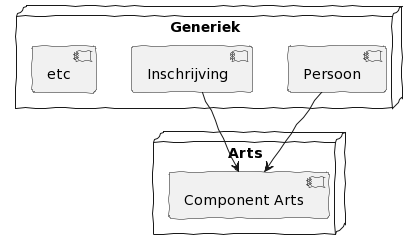
\includegraphics[width=0.4\textwidth]
        {arts.png}
     \caption{Arts with generiek}
     \label{fig:arts-deploy}
 \end{figure}
 \hfill
 \begin{figure}[h]
     \centering
     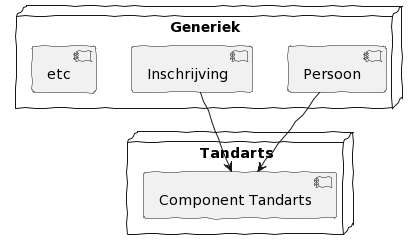
\includegraphics[width=0.4\textwidth]
        {tandarts.png}
    \caption{Tandarts with generiek}
    \label{fig:tandarts-deploy}
 \end{figure}
\\
Then the first professional group was removed from the database and the common data was also removed and the second group was fully initiated.
The method of building specific professional registers in this way is not (yet) supported by Ampersand, so it has to deployed all in once (\ref{fig:monoliet-deployment}).
\begin{figure}[H]
    \centering
        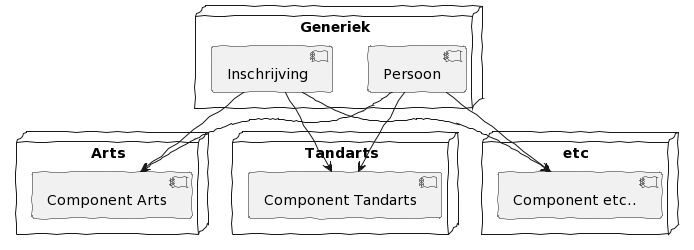
\includegraphics[width=1\textwidth]
            {monoliet.png}
        \caption{Deployment in once}
    \label{fig:monoliet-deployment}
\end{figure}
If this does not work for this law, it will also not work for links with other registers where data and the associated management software must be shared.
(Ref. to \nameref{s:3_2_common_objects})


\subsubsection{Authorization mechanism}\label{subsub:1_authorization_mechanism}
Every organization has an authorization mechanism for the software.
The \acrshort{cibg} uses a JWT mechanism.
In the research I encountered an authorization mechanism when creating the Rules and when building the Interface.
I have not found out whether it is possible to integrate this with the organization its own authorization mechanism.
(Ref. to \nameref{s:3_3_crud})


\subsubsection{Conventions}\label{subsub:1_conventions}
To use Ampersand correctly, knowledge of relation algebra is required.
You use this algebra as a Software engineer to build rules and relationships.
The knowledge of multiplicity is indispensable when making rules and relationships.
The naming convention on this is partly present within Ampersand.
Some elements, such as pattern, are capitalized and Concepts always start with a capital letter.
For example, there are a number of fixed agreements, but there are no agreements about the use of, for example, relation names.
(Ref. to \nameref{s:2_1_naming}, \nameref{s:2_2_multiplicity}, \nameref{s:2_3_rules})

\subsubsection{Other knowledge}\label{subsub:1_other_knowledge}
The Software engineer needs limited knowledge of Latex and HTML to influence the \acrshort{ca}.
In many cases this is not necessary because Ampersand handles this excellently.
However, there are opportunities to intervene and provide direction here.
(Ref. to \nameref{s:4_2_conceptual_analysis})

\subsubsection{Includes}\label{subsub:1_includes}
The Software engineer must know how to control Ampersand in terms of the use of includes.
These includes control the \acrshort{ca}, but are also used when building the application.
If the include is not specified where they are needed the build will fail and if it is specified where it is not needed the build will go well.
The \acrshort{se} has the option to send the \acrshort{ca} with includes.
The development of extra functions that have not yet been included within Ampersand is done using PHP.
The Software engineer therefore needs knowledge of PHP to develop these functions and of course Ampersand to be able to actually deploy these functions.
(Ref. to \nameref{s:3_1_includes}, \nameref{s:3_4_php})

\subsubsection{Team}\label{subsub:1_team}
The team that Ampersand maintains and wants to expand is very active.
The involvement is also apparent from the rapid resolution of issues that occurred.
(Ref. to \nameref{s:1_1_setup})

\subsection{Ampersand core in wet BIG}\label{subsection:ampersand-core-in-wet-big}
With sub-question "\acrlong{RQ2}" we want to know what is in the \acrlong{ca}.
For this appendix~\ref{appendixContentAnalysis} is included.
The \acrlong{ca} contains the Concepts, Relations and Rules (see figure~\ref{fig:LogicalDataModel}).
\begin{figure}[!htp]
    \centering
        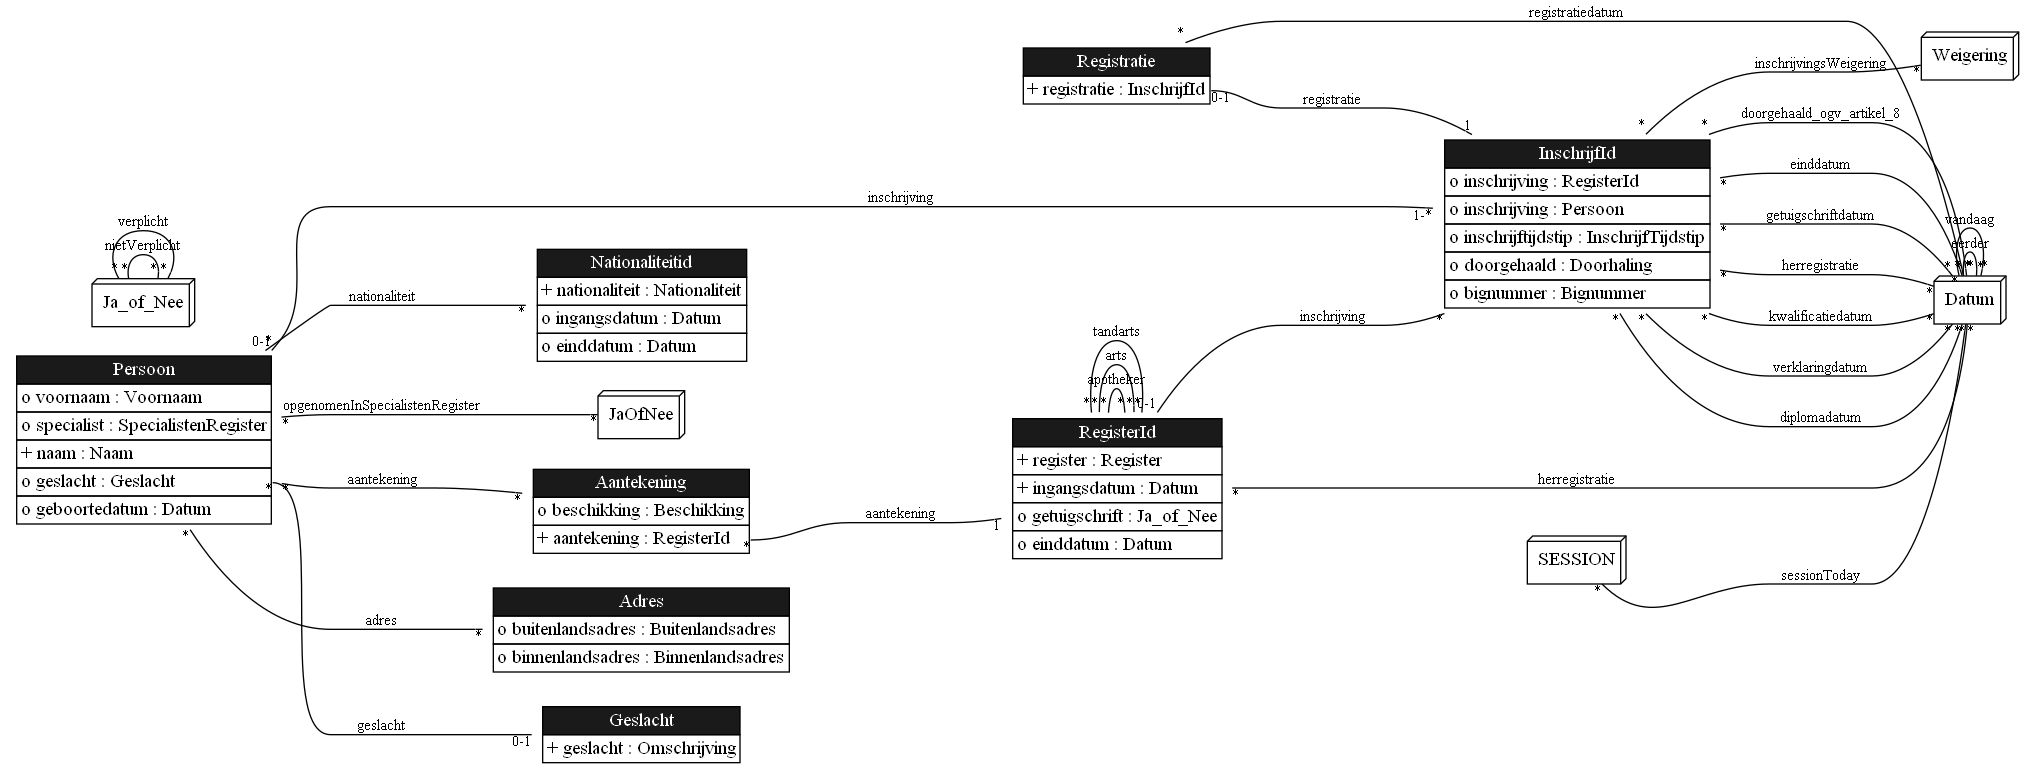
\includegraphics[width=1\textwidth]
            {../images/LogicalDataModel.png}
        \caption{LogicalDataModel from the \acrlong{ca}}
    \label{fig:LogicalDataModel}
\end{figure}
The \acrlong{ca} is not completed because not all articles and related regulations has been analyzed.
The main concepts that appear in the \acrshort{big} are Persoon, Inschrijving, Register, Arts, Tandarts, Apotheker, Gezondheidszorgpsycholoog, Psychotherapeut, Fysiotherapeut, Verloskundige, Verpleegkundige, Physician\_assistant, Orthopedagoog\_generalist, Klinisch\_technoloog, Inschrijfduur, Registratie, Weigering, Aantekening, Geslacht, Nationaliteit, Adres, Specialisme. More Concepts can be identified, but not the entire law and not all associated laws and regulations have been analysed. Not all concepts are interrelated. The Arts and Tandarts do not have a functional relationship, but they do share the relationship to Persoon and Inschrijving.

\subsection{Setup law for Ampersand}\label{subsection:setup-law-for-ampersand}
Reading and understanding the legal texts requires special skills.
For example, article 13 paragraph 1, here it reads:
\textit{"Indien bij besluit van Onze Minister inschrijving in een register is geweigerd, de afgifte van een verklaring van vakbekwaamheid wordt geweigerd of een beroepsbeoefenaar de bevoegdheid zijn beroep uit te oefenen heeft verloren omdat hij de aanvraag tot inschrijving of tot afgifte van een verklaring gebaseerd heeft op valse kwalificaties, kan Onze Minister besluiten, onverminderd de hoofdstuk V van de Algemene verordening gegevensbescherming, de bevoegde autoriteiten van andere staten dan de staten bedoeld in artikel 31a, eerste lid, van de Algemene wet erkenning EU-beroepskwalificaties, daarvan in kennis stellen."}
Due to the length of the sentences and the many parentheses, the analysis of a piece of legal text can only be read properly by a person with experience in reading legal documents.

The sub-question "\acrlong{RQ3}" deals with the law, in the case of the \acrshort{big}, and the way in which it can be analyzed and processed using Ampersand.
To answer this question we use the links as showed in table~\ref{tab:results_to_rq}.
The categories are again clustered according to the following aggregated topics. In this respect \nameref{subsub:3_complexity}, \nameref{subsub:3_define_concepts}, \nameref{subsub:3_legal_knowledge}, \nameref{subsub:3_lifecycle} and \nameref{subsub:3_structure_of_the_law}.

\subsubsection{Complexity}\label{subsub:3_complexity}
Interviews paint a picture of a law that originated in the 19th century.
Although this has been adapted to the current times, the structure is not equipped for a one-to-one translation to an information system.
It has been indicated that there are new laws that are much better suited for translation, such as, for example, "Regeling bewijsstukken sociale hygiëne Drank- en Horecawet 2015".
Since we have not analyzed any other laws, it cannot be determined whether this is the case, however the \acrshort{big} is a large and complex law, according to a lawyer at the \acrshort{cibg}.
(Ref. to \nameref{s:6_5_suitability_of_the_law})

\subsubsection{Legal knowledge}\label{subsub:3_legal_knowledge}
Analyzing the law requires legal knowledge.
Reading the legal texts also requires the necessary experience.
Analyzing the law is usually not the domain of a business analyst.
At the start of the analysis, a team should be set up that should include at least an analyst and a lawyer.
The analyst for building and managing the script and the lawyer for the translation of the law into Concepts and Relationships.
This ensures consistency and completeness of the analysis.
It has been found that even a lawyer can understand the concepts and the relationships of conceptual analysis.
As a result, the cooperation on this point will run smoothly.
(Ref. to \nameref{s:6_2_law}) 

\subsubsection{Structure of the law}\label{subsub:3_structure_of_the_law}
By starting with the analysis of the law with the help of a lawyer, an overview can be obtained at an early stage of the content and structure of the law.
By looking at the structure, the analyst can better understand what the law is about.
The structure can also help to determine the structure of the patterns.
It is certainly not the case that every chapter is a separate pattern, but it certainly influences the setup of the \acrlong{ca} and thereby help to gain an overview of the law and, on the other hand, of the analysis to be performed.
(Ref. to \nameref{s:6_4_tools}, \nameref{s:6_3_parts})

\subsubsection{Define Concepts}\label{subsub:3_define_concepts}
In order to extract the correct data and understandable data from the source text, experience is required in reading and interpreting the legal texts.
Some laws lend themselves to this better than others.
In addition to the understandable law, a law analyst is also needed.
(Ref. to \nameref{s:1_5_script_metadata}, \nameref{s:1_6_deviation})

\subsubsection{Lifecycle management within the law}\label{subsub:3_lifecycle}
The set-up of the \acrshort{big} is limited in nature, in the sense that it does not include lifecycle management.
The law regulates how a person can register and deregister.
The law also specifies the requirements that the person must meet in order to remain registered.
This is partly general and partly per register.
The missing life cycle management relates to the management of the registers themselves.
The law states that they are there, in regulations more registers are added within the \acrshort{big}, but nowhere does it say what should be done when cleaning one or more registers.
(Ref. to \nameref{s:4_3_lifecycle_law},  \nameref{s:4_4_register_unbundling})

\subsubsection{Scope}\label{subsub:3_scope}
In the first step of the analysis of an assignment in which Ampersand is used, the scope of the analysis is determined.
This scope is often more than the law itself.
In the case of \acrshort{big} there is a list of rules and decisions (see listing~\ref{list:ass-laws-regulations}).
In addition to the immediately findable legislation and regulations, there are also overarching regulations that play a role.
In some cases, it is the laws and regulations that affect the scope, but they are rules set by another source.
Such as the NORA architecture rules and the BRP address formatting rules.
It takes people from different disciplines to determine the scope.
(Ref. to \nameref{s:6_1_environment}, \nameref{s:4_6_brp})

\subsection{Ampersand for government organization}\label{subsection:ampersand-for-government-organization}
The sub-question "\acrlong{RQ4}" focuses on the use of Ampersand within the \acrshort{cibg} organization.
The information systems that are not based on legislation and regulations and which aim to monitor data quality are often the registers.
\acrshort{cibg} builds, manages and monitors this data through registration systems.

\subsubsection{Strength}\label{subsub:4_strength}
The Strength encompasses Ampersand its strengths for the \acrshort{cibg} organization.

\paragraph{\textbf{API availability}}\label{swot:s_api_availability}:
Although Ampersand is intended as a design and prototyping tool, it does have APIs at its disposal.
This can only be obtained from log lines and apparently not intended as a means of communication from external systems.
This is also apparent from the fact that no API description is made in, for example, Swagger~\footnote{\url{https://swagger.io}}, but it can work that way.
It is possible to communicate with the Ampersand core from an external source.
(Ref. to \nameref{s:1_8_api})

\paragraph{\textbf{No technical debt}}\label{swot:s_no_technical_debt}:
In conversations with an architect of the \acrshort{cibg}, the maintenance of the Ampersand model is discussed.
When a model is created, it results in a particular version of the model.
The model consists of a database model and middleware and an \acrshort{ca}, visualized using a prototype.
This model can be implemented by a development team.
Legislation will certainly be amended during the software lifecycle.
By incorporating these changes into the model, a new model is created.
The advantage of a new model is that the software does not have to do with legacy.
It is therefore always a state-of-the-art model.
(Ref. to \nameref{s:1_9_model_maintenance}, \nameref{s:4_8_user_experience})

\paragraph{\textbf{Low code}}\label{swot:s_low_code}:
Ampersand is a declarative textual language, which uses relation algebra.
The language is descriptive and eliminates the need for programming code to build the application.
Basically it should not be necessary for an \acrshort{se} to do the job.
Creating an Ampersand application can be made by a business analyst.
(Ref. to \nameref{s:3_5_model_maintenance})

\paragraph{\textbf{Reactive approach}}\label{swot:s_reactive_approach}:
Ampersand is declarative and reactive, so the Ampersand implementation always responds to the current situation through validations.
The execution of management processes is left to the \acrshort{rk}, which supports the process handling.
(Ref. to \nameref{s:5_1_registerkern})

\paragraph{\textbf{Error free specifications}}\label{swot:s_error_free_specifications}:
The Ampersand method causes the \acrshort{se} from the \acrshort{big} to create a declarative script that generates an \acrshort{ca} and a prototype.
Due to Ampersand its reactive design, the generated specifications ensure error-free implementation of the requirements.
Ampersand uses a formal language to define the specifications.
Using formal language means that system boundaries can be described, the functional behavior of the system can be defined and the system can be proven to conform to specifications (see appendix~\ref{appendixProof}).
(Ref. to \nameref{s:1_9_model_maintenance})

\paragraph{\textbf{\acrlong{ca}}}\label{swot:s_conceptual_analysis}:
The design process of an information system relies heavily on documentation.
While descriptive and analysing, the model grows.
In the case of the use of Ampersand, the basis of the realization is therefore the \acrshort{ca}.
The \acrshort{ca} can be assessed in different ways.
This can be viewed from both the business and the technology perspective.
(Ref. to \nameref{s:2_2_multiplicity}, \nameref{s:4_7_total_design})

\paragraph{\textbf{Prototype}}\label{swot:s_prototype}:
The \acrshort{ca} not only gives a description of Concepts, Relations and Rules, but also generates a logical (see figure~\ref{fig:LogicalDataModel}) and technical data model (see appendix~\ref{appendixTechDatamodel} ).
At an early stage of the realization of an information system, test scenarios can already be made on the basis of the \acrshort{ca} and these can be tested directly on the co-generated prototype.
(Ref. to \nameref{s:2_6_prototype_use}, \nameref{s:4_5_test_scenario})

\paragraph{\textbf{Team effort}}\label{swot:s_team_effort}:
To properly perform the \acrshort{big} analysis, it is not enough to have it performed by one person, as in the study.
Due to inexperience with the use of Ampersand, the first set of agreements regarding use was not made.
Ampersand knowledge is only really gained during implementation.
In addition, the amount of legal texts is so large that it cannot be read within a reasonable period of time.
In addition to IT knowledge, legal knowledge is also required, on the one hand to be able to read the law and on the other hand to find the implicitly related laws and regulations.
A team size is determined depending on the scope of the legislation and regulations to be analyzed and the lead time that one wants to use.
A team consists of at least a lawyer and an (Ampersand) experienced business analyst and a third person to validate the data.
An additional aspect is that it is possible to test for inconsistencies within the law.
It should be assumed that there are no inconsistencies but with larger and older laws this could happen.
When inconsistencies are discovered, they can be sent back to the appropriate policy directorate.
(Ref. to \nameref{s:2_5_team}, \nameref{s:1_11_law_effective}, \nameref{s:2_7_organisation_ampersand_use})

\subsubsection{Weaknesses}\label{subsub:4_weaknesses}

\paragraph{\textbf{API description}}\label{swot:w_api_its_description}:
A strong point of Ampersand is the availability of APIs.
The description and definition of the APIs would be an addition in the usage of the APIs.
Although the designed system is not intended to be used in production, APIs can be used to test against from an external source.
(Ref. to \nameref{s:1_8_api})

\paragraph{\textbf{Manual mapping}}\label{swot:w_manual_mapping}:
To link an Ampersand design to an existing system such as \acrshort{rk} mapping actions are needed.
The Ampersand design and \acrshort{rk} have similar elements.
These elements must be found and mapped onto each other.
The elements do not necessarily have the same name and if they already have the same name, the definition may differ.
The manual mapping is a design point of attention and measures will have to be taken to identify it.
The agreement could be to detect this already during the design and have a comment about this included in the \acrshort{ca}.
(Ref. to \nameref{s:4_1_architectural_fit}, \nameref{s:1_7_architecture_and_registerkern}, \nameref{s:5_2_demarcation})

\paragraph{\textbf{Data migration}}\label{swot:w_data_migration}:
Ampersand does not provide any resources to guide the conversion from the old model to the new model.
The development team will therefore have to make an analysis of the old and the new situation and have to develop conversion software for that.
This is a method that is different from usual.
The downside is that the conversion is likely to be complex.
Data that was previously valid may be invalid in a subsequent model.
(Ref. to \nameref{s:3_5_model_maintenance})

\paragraph{\textbf{Documentation }}\label{swot:w_documentation}:
During the setup and use of Ampersand, we often fall back on the available documentation of the tool.
The documentation is mainly available on the formal Ampersand site (\footnote{\url{https://ampersandtarski.gitbook.io/documentation/}} and very little on other sites.
A common method is, for example, to perform a search in which a question is specified.
Because Ampersand is not widely used, there is not much support on the internet and you can only fall back on the formal site and the examples that are available on github.
This sometimes makes it difficult to resolve an issue.
(Ref. to \nameref{s:1_1_setup}, \nameref{s:3_3_crud})


\subsubsection{Opportunities}\label{subsub:4_opportunities}


\paragraph{\textbf{API http-code response}}\label{swot:o_api_http_responsecode}:
The return actions from the called APIs are not provided with a code but text.
As proof of concept, calls were made from Postman~(see figure~\ref{fig:postman-get-person}) to Ampersand and that worked as expected.
(Ref. to \nameref{s:1_8_api})
\begin{figure}[ht]
    \centering
    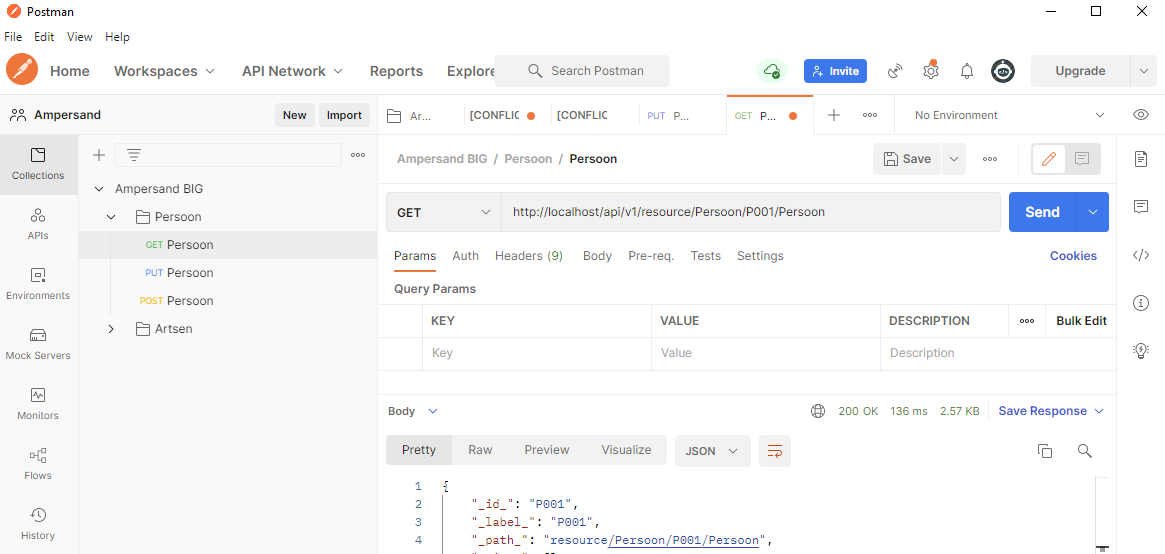
\includegraphics[width=\textwidth]{/postman_GET.PNG}
    \caption{Postman GET Person}
    \label{fig:postman-get-person}
\end{figure}

\paragraph{\textbf{Customization \acrshort{rk}}}\label{swot:o_customization}:
An organized ICT organization such as the \acrshort{cibg} has an architecture that new software must comply with.
One of the developments in the \acrshort{cibg} is the set-up of the \acrshort{rk} (see interview developer Appendix~\ref{par:interview-developer}).
\acrlong{rk} its terminology includes "zaken" and "producten".
Every service, read implementation of a law, we call a product.
There are default items that always appear in every registry.
These are pre-modeled in \acrshort{rk}.
This includes a foundation for each registry and can be expanded to meet the needs of the registry.
The basis is the minimum common denominator of the registers, extendable to specific elements arising from the law.
There is certainly overlap in the data obtained from the analysis of the great law and the \acrshort{rk}.
About 80\% of the \acrshort{rk} is generic and the other 20\% is custom.
All new registers therefore have the same basic principles and largely run on the same software.
However, a mapping still has to take place from the found Concepts from the law to \acrshort{rk}.
The overlap in this is not always immediately visible.
Within the \acrshort{rk} the term product is used, within the \acrshort{big} this product is a register or possibly even all registers.
The latter depends on the implementation.
This mapping must be made explicit and has not been taken into account in this study.
The developer has indicated that full integration of the Ampersand model is not possible, due to the aforementioned overlap of the Concepts.
However, the modified part of the \acrshort{rk} can be used for the Ampersand model implementation.
Although Ampersand is new to the \acrshort{cibg} organization, one of the interviewees pointed out (see interview analist~\ref{par:interview-analist}) that documentation in the form of a design should be made with each new register.
According to the analyst, it should not matter which tool is used for this.
The advantage of Ampersand is that it generates a model from the analysis instead of the usual model-to-text approach.
A model is made of each pattern.
See for example the Pattern for \mbox{Person} (see script~\ref{lst:persoon}).
This results in the model of figure~\ref{fig:pattern-persoon}.
\begin{figure}[H]
    \centering
        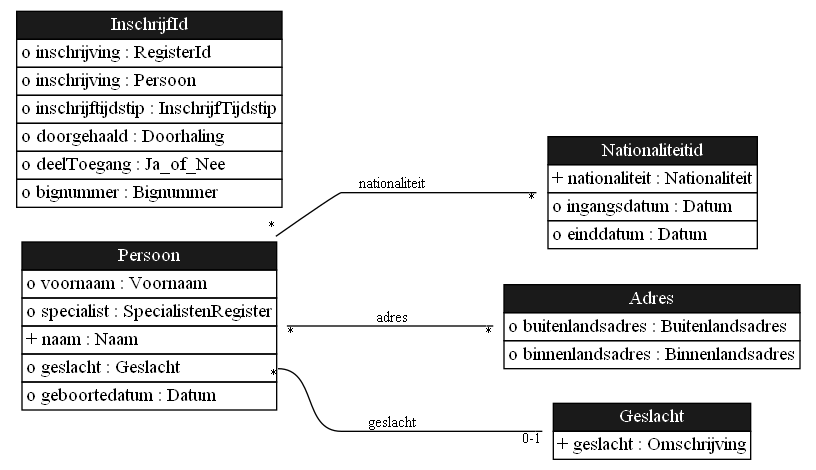
\includegraphics[width=1\textwidth]
            {../images/CDPatternPersoon.png}
        \caption{Pattern Persoon}
    \label{fig:pattern-persoon}
\end{figure}
Calculations are not standard in Ampersand, but this can be solved by writing external functions or even solving it in \acrshort{rk}.
(Ref. to  \nameref{s:5_2_demarcation}, \nameref{s:1_7_architecture_and_registerkern}, \nameref{s:4_1_architectural_fit}, \nameref{s:1_10_ampersand_design_method}, \nameref{s:2_7_organisation_ampersand_use}, \nameref{s:4_7_total_design})

\paragraph{\textbf{Version-gap analysis}}\label{swot:o_version_gap_analysis}:
Although it is not the intention to use Ampersand prototype in a production environment, it is useful to save the data entered in an earlier version and use it in later versions.
In ``\nameref{swot:w_data_migration}'' included with the weaknesses we indicate that this is a problem and it would be a good addition to develop a tool in Ampersand that focuses on preserving data across versions.
(Ref. to \nameref{s:3_5_model_maintenance})

\paragraph{\textbf{Atlas local}}\label{swot:o_atlas_local}:
In RAP there is a tool called Atlas, it shows the context and the patterns.
In addition, all Concepts, Rules, Properties and Relations, with hyperlinks to the components.
Via the hyperlink details of the item inclusion a relationship diagram is shown, very nicely executed and very useful when working in RAP.
This tool is a viewer on the information and it is not possible to also edit the \F{information in Atlas}{Being able to edit the Atlas information from Atlas}.
However, the case study was so large that the RAP environment was not sufficient.
RAP does not support Includes and has been used extensively.
Unfortunately, \F{Atlas availability}{Make Atlas available outside the RAP environment.} cannot be implemented outside of RAP.

As a novice user of Ampersand it takes a while to master Relation algebra.
That is why an excel sheet has been made to make the Relations visible with the associated multiplicity.
This is a method that is easy to use initially.
The disadvantage of this approach is the consistent transfer of Concepts and Relations.
We need to double track this information and redundancy in the field of data will certainly go wrong.
When Concepts disappear, they must also be removed from Excel or Relations that do change due to new insights must be adjusted here.
In short, this does work for small, well-arranged projects, but for larger ones, gaps will quickly arise and this no longer represents reality.
The result was that the excel sheet was used a lot in the beginning and not anymore later on.
(Ref. to \nameref{s:3_5_model_maintenance}, \nameref{s:2_2_multiplicity})

\paragraph{\textbf{\acrlong{ca} as testbasis}}\label{swot:o_ca_as_testbasis}:
By using Ampersand as a design tool, a prototype is available at an early stage.
This prototype can be converted into a website with the appearance of a \acrshort{cibg} website by means of HTML additions and CSS adjustments.
Test cases can already be developed at an early stage on the basis of this prototype and the functions of the prototype, by using the APIs, can be used as a stub in the development of the system.
(Ref. to \nameref{s:2_6_prototype_use}, \nameref{s:1_10_ampersand_design_method})

\paragraph{\textbf{Stub}}\label{swot:o_stub}:
The prototype can be accessed through APIs.
In principle it is possible to use the prototype in whole or in part as a stub.
When developing the application, based on the \acrshort{ca}, the prototype can be used in the form of a stub.
(Ref. to \nameref{s:4_5_test_scenario})


\paragraph{\textbf{Annotation}}\label{swot:o_annotation}:
To maintain an overview when performing the textual analysis, it is necessary to use a annotation (see section~\ref{subsection:ampersand-knowledge}, heading~\nameref{subsub:1_annotation}).
Annotation would be a nice addition to Ampersand.
It does introduce a close link between Ampersand and the source document.
(Ref. to \nameref{s:1_3_source_handling})

\subsubsection{Threats}\label{subsub:4_treaths}

\paragraph{\textbf{NIH}}\label{swot:t_nih}:
Ampersand is a completely new method for the \acrshort{cibg} organization.
People have never heard of it and unfortunately there is not much to be found about it.
That means that people are not positive about it in advance, and NIH calls it~\footnote{not invented here}\citep{antons_assessing_2017}.
The expectation of the organization is that the Ampersand method will take more time than the current method (see interview~\ref{int:I-1.8}) and people will be wary of something new.
Obviously, the advantages of the method are not yet understood.
Benefits such as working directly at the source, generating a prototype from there (see appendix~\ref{appendixPrototype}) with all validations and full conceptual specifications (see appendix~\ref{ConceptualAnalysis}).
Having a prototype makes it possible to build test scenarios at an early stage and with the \acrlong{ca} you can start building right away.
(Ref. to \nameref{s:4_5_test_scenario}, \nameref{s:2_6_prototype_use}, \nameref{s:1_11_law_effective})

\paragraph{\textbf{Process orientation}}\label{swot:t_process_orientation}:
Many organizations are process oriented.
With \acrshort{cibg}, the work instructions that the employees use are usually process steps that must be performed.
Also the design of systems such as \acrshort{zorro} are designed to support a process-oriented approach.
Ampersand supports a reactive focused approach.
This cannot be translated into process-oriented work instructions.
The challenge for the adoption of Ampersand therefore lies partly in the organization its ability to adapt from process-based to reactive.
Also contributing to this is that the adjacent system, \acrshort{rk}, is a process-oriented system, which supports a number of standard processes that affect (almost) every register.
(Ref. to \nameref{s:1_7_architecture_and_registerkern}, \nameref{s:5_1_registerkern}, \nameref{s:5_2_demarcation})

\paragraph{\textbf{Redundancy}}\label{swot:t_redundancy_script_tool}:
The reuse of Concepts, Relations and Rules is on the one hand a powerful means whereby consistency is enforced.
However, when using Ampersand, it is not always visible that components are already being used.
For example, it is possible to include these components several times in the analysis and to assign them a different definition each time.
While this should be detectable by Ampersand.
Conversely, it is also possible to rename components with the same definition.
Of course, Ampersand cannot control this.
The IDE used should support this, but it does not at the moment.
(Ref. to \nameref{s:5_2_demarcation})

\paragraph{\textbf{IDE-refactoring}}\label{swot:t_ide_refactoring}:
Ampersand as a tool is supported by an IDE.
For \acrshort{vsc} there is a plugin that supports the use of Ampersand.
In addition, the Ampersand tool is built in such a way that the compilation of the script from the \acrshort{vsc} is supported.
An omission in the use of \acrshort{vsc} is a refactoring option.
To be able to refactor, the IDE tool needs to know which components are used and where they are used.
This condition is not met, where refactoring is not possible in advance.
Not being able to refactor is a cause of causing redundancy in the code (see paragraph~\nameref{swot:t_redundancy_script_tool}).
(Ref. to \nameref{s:3_2_common_objects})





\newpage
\parindent0em
\begin{figure}[ht]
    \centering

    \begin{tikzpicture}[
        pentagon/.style={%
            shape=regular polygon, regular polygon sides=5, minimum size=7.3cm, inner
            sep=-1mm, draw, fill=lightgray!75!yellow
        }, font=\scriptsize\sffamily, thick
    ]
    
    % \draw[help lines] (-16,-16) grid (16,16);
    \filldraw[thin,gray,fill=gray!25] (-8,-8) rectangle (8,8);
    \filldraw[thin,gray,fill=white] (-7.15,-7.15) rectangle (7.15,7.15);
    \draw[thin,gray] (7.15,7.15)--(8,8) (-7.15,7.15)--(-8,8) (-7.15,-7.15)--(-8,-8)
    (7.15,-7.15)--(8,-8);
    
    % Strengths
    \draw[thin,gray] (-0.025,0.025)--(-7.05,0.025)--(-0.025,7.05)--cycle;
    \node[pentagon,rotate=0] at (-3.75,3.75) {
        \begin{varwidth}{\linewidth}
            \begin{itemize}[leftmargin=*,noitemsep]
                \item \nameref{swot:s_api_availability}
                \item \nameref{swot:s_prototype}
                \item \nameref{swot:s_no_technical_debt}
                \item \nameref{swot:s_low_code}
                \item \nameref{swot:s_reactive_approach}
                \item \nameref{swot:s_error_free_specifications}
                \item \nameref{swot:s_conceptual_analysis}
                \item \nameref{swot:s_team_effort}
            \end{itemize}
        \end{varwidth}
    };
    \draw (-4,2) node[rotate=0] {\large\textbf{Strengths}};
    
    % Weaknesses
    \draw[thin,gray] (0.025,0.025)--(7.05,0.025)--(0.025,7.05)--cycle;
    \node[pentagon,rotate=0] at (3.75,3.75) {
        \begin{varwidth}{\linewidth}
            \begin{itemize}[leftmargin=*,noitemsep]
                \item \nameref{swot:w_api_its_description}
                \item \nameref{swot:w_manual_mapping}
                \item \nameref{swot:w_data_migration}
                \item \nameref{swot:w_documentation}
            \end{itemize}
        \end{varwidth}
    };
    \draw (4,2) node[rotate=0] {\large\textbf{Weaknesses}};
    
    % Opportunities
    \draw[thin,gray] (-0.025,-0.025)--(-7.05,-0.025)--(-0.025,-7.05)--cycle;
    \node[pentagon,rotate=0] at (-3.75,-3.75) {
        \begin{varwidth}{\linewidth}
            \begin{itemize}[leftmargin=*,noitemsep]
                \item \nameref{swot:o_api_http_responsecode}
                \item \nameref{swot:o_customization}
                \item \nameref{swot:o_version_gap_analysis}
                \item \nameref{swot:o_atlas_local}
                \item \nameref{swot:o_ca_as_testbasis}
                \item \nameref{swot:o_stub}
                \item \nameref{swot:o_annotation}
            \end{itemize}
        \end{varwidth}
    };
    \draw (-4,-2) node[rotate=0] {\large\textbf{Opportunities}};
    
    % Threats
    \draw[thin,gray] (0.025,-0.025)--(7.05,-0.025)--(0.025,-7.05)--cycle;
    \node[pentagon,rotate=0] at (3.75,-3.75) {
        \begin{varwidth}{\linewidth}
            \begin{itemize}[leftmargin=*,noitemsep]
                \item \nameref{swot:t_nih}
                \item \nameref{swot:t_process_orientation}
                \item \nameref{swot:t_redundancy_script_tool}
                \item \nameref{swot:t_ide_refactoring}
            \end{itemize}
        \end{varwidth}
    };
    \draw (4,-2) node[rotate=0] {\large\textbf{Threats}};
    \draw(0,-7.55) node {\Large EXTERNAL};
    \draw(0,7.55) node {\Large INTERNAL};
    \draw(-7.55,0) node[rotate=90] {\Large POSITIVE};
    \draw(7.55,0) node[rotate=270] {\Large NEGATIVE};
    \draw(-0.6,0.6) node {\Huge\textbf{S}}; 
    \draw(0.6,0.6) node {\Huge\textbf{W}};
    \draw(-0.6,-0.6) node {\Huge\textbf{O}};
    \draw(0.6,-0.6) node {\Huge\textbf{T}};
    \end{tikzpicture}
    \caption{SWOT Ampersand for government organization}
    \label{fig:swot}
\end{figure}

\parindent2em

The design of register systems has no specific points for attention.
Part of the research question was about designing for register systems.
Other than the source specific link, the \acrshort{big}, no particulars were found for registry systems.
The translation of this law into an information system results in a register.
The requirements of the register are laid down by law.
This concerned, among other things, the identifying data of a registration and in Article 3, paragraph 1~\footnote{\url{https://wetten.overheid.nl/jci1.3:c:BWBR0006251&hoofdstuk=II&paragraaf=1&article=3&z=2022-04-01&g=2022-04-01}} it says it is about multiple registers.
This also explains why there are few observations about registration systems.
The register system therefore does not stand alone, but is a consequence of the fact that the source is a law.

\subsection{Limitions}\label{sbs:limitions}
The focus of the research was on executing the process to construct at a \acrshort{ca} and a prototype.
The time for this is in principle 26 weeks.
We have moved a little over time and it turns out that it is not possible to fully analyze just a law like \acrshort{big}.
The limitation we encountered is that there is a shortage of time.
This has to do with an optimistic estimate of what work can be done.
The start with Ampersand is more difficult than it seems.
The \acrshort{big} is much larger and more complex than it first appears.
Reading the law is also an art.
The law has many references to other laws.
This resulted in an \acrshort{ca} which is not complete.
The process did provide enough material to make several statements (see section~\ref{conclusions})

\begin{comment}
discussie voer

niet alle observaties zijn gebruikt

Een risico dat gelopen wordt door de moeilijke teksten is dat er niet zorgvuldig genoeg gelezen wordt en er eigen interpretatie plaatsvindt.
Dat risico neemt toe, naar mate het domein vertrouwder is voor de onderzoeker. 
Dus de keerzijde van de \acrshort{ar} aanpak is een bias op de inhoud.

De overall aanpak van de analyse van de wet is om eerst een overzicht te krijgen van de wet.
Het doorlopen van de wet en de highlights van de artikelen helder te krijgen.
Dit sluit aan bij het idee om de indeling op voorhand te maken


Vanuit verschillende interviews werd het statement gemaakt of \acrshort{big} wel de meest geschikte wet is om deze met Ampersand te analyseren.
Reden is dat de wet van orgine heel oud is~\ref{section:big}. 
De wet is verschillende malen bijgewerkt, maar de structuur is niet simpel om te zetten naar een ICT-systeem.
Daarnaast bevat de wet zeer veel impliciete en expliciete verwijzingen naar andere wet- en regelgeving.
En de wet is zelf niet expliciet genoeg.
Er zijn behoorlijk veel interpretatie mogelijkheden.
-> leidt tot sneller aansluiten bij de tot stand koming van de wet
-> vroegtijdige analyse van de haalbaarheid
-> alternatieve aanpak etc.
\end{comment}



\addtocontents{toc}{\protect\setcounter{tocdepth}{3}}

